%- - - - - - - - - - - - - - - - - - - - - - - - - - - - - - - - - PROBLEMAS AD HOC -
%- - - - - - - - - - - - - - - - - - - - - - - - - - - - - - - - - SLIDE -
\begin{frame}
\frametitle{Problemas Ad Hoc}
\begin{block}{O que são?}
\begin{itemize}
	\bitem Problemas ``Ad Hoc'' são aqueles cuja solução não utiliza nenhum algoritmo bem conhecido.
	\bitem Cada problema ``Ad Hoc'' é diferente e tem uma solução específica.
	\bitem Geralmente esses problemas são os mais divertidos (e as vezes os mais frustrantes) já que cada um apresenta um novo desafio.
	\bitem A solução pode envolver uma estrutura de dados singular ou um conjunto incomum de loops e/ou condicionais.
	\bitem Não exclui o uso de outras técnicas.
\end{itemize}
\end{block}
\end{frame}
%- - - - - - - - - - - - - - - - - - - - - - - - - - - - - - - - - SLIDE -
\begin{frame}
\frametitle{Problemas Ad Hoc}
\begin{center}
	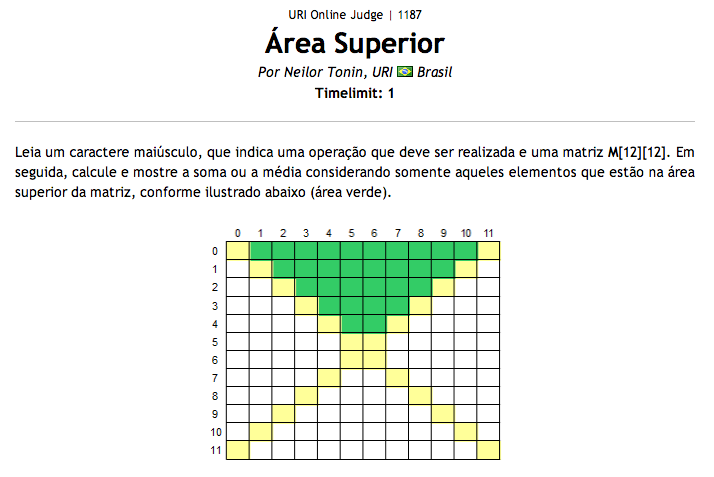
\includegraphics[width=.85\textwidth]{figuras/URI-1187.png}
\end{center}
\end{frame}	
